%!TeX program = xelatex
\documentclass{SYSUReport}
\usepackage{booktabs}

%设置列表的间距
\usepackage{enumitem}
\setenumerate[1]{itemsep=2pt,partopsep=0pt,parsep=\parskip,topsep=5pt}    %itemsep即列表中两行间距
\setitemize[1]{itemsep=2pt,partopsep=0pt,parsep=\parskip,topsep=5pt}

% 根据个人情况修改
\headl{}
\headc{}    %中间页眉
\headr{}
\lessonTitle{数学建模课程报告}
\reportTitle{饮食计划研究}
\stuname{{\CJKfontspec{楷体} 陈大文}}    %自定义字体
\stuid{2021100xxxx} 
\inst{计算机学院}
\major{大数据}
\date{2023年11月22日}

\begin{document}

% =============================================
% Part 1: 封面
% =============================================
\cover
\thispagestyle{empty} % 首页不显示页码
\clearpage

% =============================================
% Part 2: 摘要
% =============================================
%\begin{abstract}
%
%在此填写摘要内容
%
%\end{abstract}
% \thispagestyle{empty} % 摘要页不显示页码
% \clearpage


% =============================================
% Part 3: 目录页
% =============================================
% 重置页码,并使用罗马数字
\pagenumbering{Roman}
\setcounter{page}{1}
\tableofcontents
\clearpage

% =============================================
% Part 4: 正文内容
% =============================================
% 重置页码,并使用阿拉伯数字
\pagenumbering{arabic}
\setcounter{page}{1}

%%可选择这里也放一个标题
%\begin{center}
%    \title{ \Huge \textbf{{标题}}}
%\end{center}

\section{提出问题}
\subsection{问题描述}

合理的饮食是身体健康的基础。科学的控制摄入食物的比例可以健康的减肥。实际的饮食计划中既要考虑较低的热量摄入,还要考虑较高的满足感和饱腹感,并且营养要均衡。现在需要对饮食计划进行建模,求出一个人每天的饮食安排(即每种食物一天的摄入量),要求:
\begin{enumerate}
    \item 只考虑饮食,不考虑运动,假设基础代谢为常数。    \vspace{-0.3cm}
    \item 只考虑食物中的主要成分:蛋白质,脂肪,碳水化合物三种主要热量来源,考虑维生素,钠离子两种微量元素,不考虑其它微量元素。    \vspace{-0.3cm}    
    \item 饮食计划要综合考虑:热量摄入、饱腹感(GI值)、满足感(假设依赖于脂肪和糖)。    \vspace{-0.3cm}
\end{enumerate}

\subsection{问题背景}
\subsubsection{基础代谢率(BMR)}
基础代谢率(Basal Metabolic Rate,BMR)是指人体在清醒而又极端安静的状态下,不受肌肉活动、环境温度、食物及精神紧张等影响时的能量代谢率。即进行基本的生理活动(血液循环、呼吸及恒定的体温)时,每小时单位表面积最低耗热量减去标准耗热量,其差值与标准耗热量之百分比,称为基础代谢率。

如果想要使用较容易获得的参数,精确的计算BMR,可以参考以下基础代谢率公式:
\begin{equation*}
    BMR = \begin{cases} 
66 + (13.7 \times w) + (5 \times h) - (6.8 \times a) & \text{(男性)} \\
655 + (9.6 \times w) + (1.8 \times h) - (4.7 \times a) & \text{(女性)}
\end{cases}
\end{equation*}

其中, $w$为体重(单位:kg), $h$为身高(单位:cm), $a$为年龄(单位: 年)。

\subsubsection{主要热量来源}
食物一般由碳水化合物、蛋白质、脂肪这三种物质组成,它们是人的主要热量来源,产生的热能为:

\begin{table}[h!]
\centering
\renewcommand\arraystretch{0.65}
\begin{tabular}{ll}
\toprule
		热量来源  & 热能   \\ \midrule
		碳水化合物 & 4千卡/克  \\
		蛋白质   & 4千卡/克  \\
		脂肪    & 9千卡/克  \\ 
\bottomrule
\end{tabular}
\caption{营养物质摄入参考表}
\label{heat-table}
\end{table}
根据《中国居民膳食指南(2022)》,蛋白质摄取量应为人体每日所需热量的10$\%$~15$\%$;碳水化合物摄取量应为人体每日所需热量的 50$\%$~65$\%$;脂肪的摄取量应为每日所需热量的20$\%$~30$\%$。

\subsubsection{微量元素摄入}
依题意,此处只考虑维生素,钠离子两种微量元素。

维生素 (Vitamin) 是人维持正常的生理功能而必须从食物中获得的一类微量有机物质,在人体生长、代谢、发育过程中发挥着重要的作用。维生素在体内既不参与构成人体细胞,也不为人体提供能量。维生素参与人体的生化反应,调节人体的代谢功能,如果维生素摄入不足,会导致人体新陈代谢失去平衡,会导致免疫力下降并可能导致营养不良,易患各种疾病。

成人一天需要摄入的各种维生素的量如下:
\begin{table}[h!]
\centering
\renewcommand\arraystretch{0.6}
\scalebox{0.7}{
\begin{tabular}{cccccccccccc}
\toprule
\quad & 维生素 A & 维生素 B1 & 维生素 B2 & 维生素 B6 & 维生素 B12 & 维生素 C & 维生素 E & 尼克酸 & 叶酸 & 泛酸\\ 
\midrule
需求量 & 2mg & 1.4mg & 1.6mg & 2mg & 1μg & 60mg & 10mg & 18mg & 200μg & 6mg  \\
\bottomrule
\end{tabular}}
\caption{营养物质摄入参考表}
\label{vitamin-table}
\end{table}

钠离子对人体有调节和控制作用。人类在长期出汗过多、腹泻、呕吐及肾上腺皮质不足等情况下,会发生钠缺乏症。钠缺乏症可造成生长缓慢、食欲减退、由于失水体重减轻、哺乳期的母亲奶水减少、肌肉痉挛、恶心、腹泻和头痛。膳食中长期摄入过多的钠将导致高血压,如果误将食盐当作食糖给婴幼儿食用,有可能导致死亡。

成年人的建议钠摄入量为\underline{2000 - 2500 mg(此处按2000mg算)}。

\subsubsection{食品摄入建议总结}
查资料可知蛋白质和碳水饱腹感高于脂肪,因此将三者单位质量饱腹感的值设为
3:1:3。而脂肪与碳水的满足感要高于蛋白质,因此将三者单位质量满足感的值设为
2:3:3。

根据上面的背景材料,可以总结得到以下表格:

\begin{table}[h!]
\centering
\renewcommand\arraystretch{0.65}
\begin{tabular}{cccccc}
\toprule
\quad & 蛋白质 & 脂肪 & 碳水化合物 & 维生素 & 矿物质 \\
\midrule
摄入占比 & 10\%--15\% & <30\% & >55\% & 0 & 0 \\
热量热量 & 4 kcal/g & 9 kcal/g & 4 kcal/g & 0 & 0 \\
比例配额 & 3 & 1 & 3 & 0 & 0 \\
营养素 & 2 & 3 & 3 & 1 & 1 \\
\bottomrule
\end{tabular}
\caption{营养物质摄入参考表}
\label{nutrients-table}
\end{table}

\section{题目假设}
    \begin{enumerate}
        \item 只考虑饮食,不考虑运动,假设基础代谢为常数。    \vspace{-0.3cm}
        \item 只考虑食物中的主要成分:蛋白质,脂肪,碳水化合物三种主要热量来源。    \vspace{-0.3cm}
        \item 考虑维生素,钠离子两种微量元素,不考虑其它微量元素。    \vspace{-0.3cm}
        \item 假设食物可以由营养素线性表出,没有损失。    \vspace{-0.3cm}
        \item 食物只考虑牛肉,羊肉,猪肉,鱼,鸡蛋,大白菜,牛奶,土豆,盐,米饭。    \vspace{-0.3cm}
    \end{enumerate}

\section{模型建立}
\subsection{模型构思}
本题要在已知的约束条件下,摄入最少的热量,其次是要获得较高的满足感和饱腹感。

根据题意,本题是一个多目标规划\cite{csdn_blog_post}问题,需要考虑三个目标:摄入最少的热量、获得较高的满足感和饱腹感,并且要满足已知的约束条件。

在本题,由于目标同时存在求最小值和求最大值问题,加权法不适用,因此我采用优先级法求解此规划问题,优先级法先求解优先级高的目标,再将求解结果代入次优先目标进行求解,以此类推,直至所有目标都求解完成。

在此处,可以优先考虑热量摄入最少,然后再考虑较高的满足感和饱腹感,因此目标优先级从高到低依次为热量摄入最少、满足感最高、饱腹感最高。

\subsection{模型建立}
该规划问题的目标为摄入的热量最少,获得尽量高的满足感和饱腹感。则目标函数如下:
\begin{equation}
\min \sum_{i=1}^{n} m_i H_i
\end{equation}

\begin{equation}
\max \sum_{i=1}^{n} m_i Sa_i
\end{equation}

\begin{equation}
\max \sum_{i=1}^{n} m_i Ful_i
\end{equation}

\textbf{其中,$n$为食物种数(此处为9),$m_i$为饮食策略中第$i$种食物食用的质量,$H_i$为第$i$种食物的单位热量,$Sa_i$为第$i$种食物单位质量贡献的满足感,$Ful_i$为第$i$种食物单位质量贡献的饱腹感。此处要求规划达到最优时所有的值。}

而根据题意,本规划问题有以下的约束条件:
\begin{itemize}
    \item BMR是人类静止的情况下热量的代谢率,如果长期摄入热量小于代谢率,人就会营养不良,因此,摄入的热量要不低于BMR,即:
\begin{equation*}
\sum_{i=1}^{n} m_i H_i \geq BMR
\end{equation*}        \vspace{-0.1cm}
    \item 蛋白质摄取量应为人体每日所需热量的10$\%$~15$\%$;,即:
\begin{equation*}
\sum_{i=1}^{n} m_i M_\text{蛋白质} \geq 0.1 \times BMR
\end{equation*}
\begin{equation*}
\sum_{i=1}^{n} m_i M_\text{蛋白质} \leq 0.15 \times BMR
\end{equation*}        \vspace{-0.1cm}
    \item 脂肪摄取量应小于人体每日所需热量的30$\%$;,即:
\begin{equation*}
\sum_{i=1}^{n} m_i M_\text{脂肪} \leq 0.3 \times BMR
\end{equation*}        \vspace{-0.1cm}
    \item 碳水化合物摄取量应不少于人体每日所需热量的55$\%$;,即:
\begin{equation*}
\sum_{i=1}^{n} m_i M_\text{碳水化合物} \geq 0.55 \times BMR
\end{equation*}        \vspace{-0.1cm}
    \item 由上面的背景知识可知,人的各种维生素摄取量总共约100mg,即:
\begin{equation*}
m_\text{维生素} = 100mg = 0.1g
\end{equation*}
    \item 人的钠摄取量约2000mg,即:
\begin{equation*}
m_\text{钠} = 2000mg = 2g
\end{equation*}        \vspace{-0.1cm}
\end{itemize}

\textbf{上述约束条件中,$M_\text{(营养元素)i}$为第i种食物种某种营养元素的含量(单位:g),$H_\text{(营养元素)}$为第该营养元素单位质量中所含的热量(单位:kcal/g)。}

\textbf{此处所有的质量m都使用g做单位,统一量纲。}

\section{模型求解}
\subsection{求解概述}
我使用python语言对此题进行求解,在python中我选择使用groubipy库作为我的求解器。Groubi\cite{gurobi_zhihu}是一个商业求解器,其具有求解精度高,代码易读性较好的优点。在此处,我使用了groubi中的\texttt{setObjectiveN}函数添加目标函数,它可以直接对不同目标设置优先级,从而自动使用优先级法进行求解。接下来使用\texttt{addConstr}函数添加约束条件,groubi中的约束条件可以直接用不等式表示,更加易读。

\subsection{需要考虑食物的营养元素含量}
此处,我使用pandas库来读取此处规划中需要考虑的各种食物中营养元素的含量表,此表中的数据来自于\textit{中国营养学会}\cite{china_nutrition_society},该表中的内容如下:

\begin{table}[h!]
\centering
\renewcommand\arraystretch{0.65}
\begin{tabular}{cccccc}
\toprule
\quad & 蛋白质 & 脂肪 & 碳水化合物 & 维生素 & 矿物质 \\
\midrule
牛肉 & 0.199 & 0.042 & 0.02 & 0 & 0.842 \\
鸡肉 & 0.19 & 0.15 & 0 & 0 & 0.806 \\
猪肉 & 0.132 & 0.37 & 0.024 & 0 & 0.594 \\
鱼 & 0.166 & 0.052 & 0.001 & 0 & 0.46 \\
水果 & 0.13 & 0.09 & 0.028 & 0.00234 & 1.315 \\
大豆类 & 0.015 & 0.001 & 0.032 & 0.31 & 0.575 \\
其他 & 0.03 & 0.032 & 0.034 & 0.01024 & 0.372 \\
乳品 & 0.02 & 0.002 & 0.172 & 0.027 & 0.027 \\
酒 & 0 & 0 & 0 & 0 & 393.11 \\
米饭 & 0.074 & 0.008 & 0.779 & 0 & 0.038 \\
\bottomrule
\end{tabular}
\caption{单位质量食物营养元素含量表}
\label{table:nutrient_intake}
\end{table}

其中,维他命和钠离子含量的单位是\textbf{毫克每克(食物)},其他营养元素含量的单位是克每克(食物)。表格存储在\texttt{diet\_plan\_my.csv}文件里,在python中使用pandas库的\texttt{read\_csv}函数导入。

\subsection{使用python进行求解}
此处使用优先级法进行求解,求解的目标设置为[c\_heat, c\_sat, c\_gi],优先级设置为3, 2, 1,分别传入\texttt{solve\_multiobjective\_linear\_program}函数中,该函数中调用groubi的setObjectiveN函数,根据传入的目标和对应的优先级设置好目标,接着添加对应的限制条件,最后对model进行optimize,求解得到结果。

规划中需要用到人的BMR,此处代入我的情况进行计算,\textbf{我的身高178cm,体重69kg,性别男,年龄20岁,得到BMR的值为1543.8}。

求解规划问题时,按优先级依次添加三个目标进行计算,计算的中间结果如下图:
\begin{figure}[h]
	\centering
	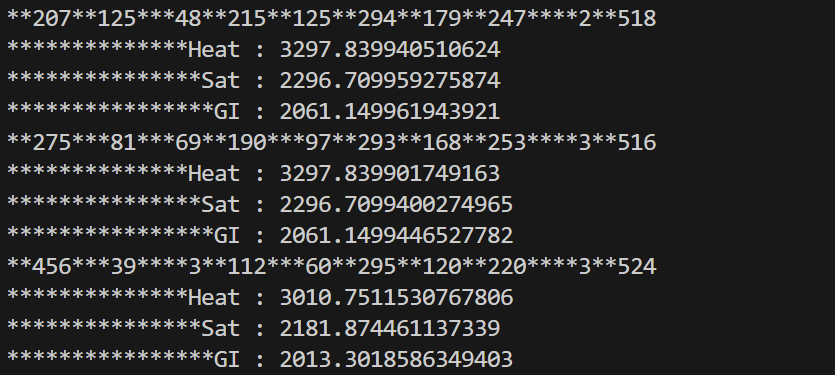
\includegraphics[width=0.6\linewidth]{figures/fig1.png}
	\caption{计算的中间结果}
	\label{mid-result-fig}
\end{figure}

可见第一次以最大化满足感为目标获得的结果分别是热量摄入3297kcal,2296,2061。这里的热量摄入是三次中最高的。然后将满足感作为条件加入已有的约束,并以最大化饱腹感为目标获得的结果是3297kcal,2296,2061,再将其加入约束,计算最小热量摄入,得到的结果为3010kcal,2181,2013。可见热量摄入较前两次有明显的减少,但代价是饱腹感和满足感的减少,且减少的幅度都在约束范围内。

所以最终的结果是最小摄入量3010kcal,最大饱腹感2181,最大满足感2013。

优化完成,得到每种食物每天的理想摄入量如下:
\begin{table}[h!]
\centering
\renewcommand\arraystretch{0.65}
\begin{tabular}{cc}
\toprule
食物种类 & 摄入量 (g) \\
\midrule
牛肉 & 456 \\
鸡肉 & 39 \\
猪肉 & 3 \\
鱼 & 112 \\
水果 & 60 \\
大豆类 & 295 \\
其他 & 120 \\
乳品 & 220 \\
酒 & 3 \\
米饭 & 524 \\
\bottomrule
\end{tabular}
\caption{摄入量食物表}
\label{food-intake-table}
\end{table}

即牛肉每天食用456g,羊肉每天食用39g,猪肉每天食用3g(相当于不吃),鱼肉每天食用112g,鸡蛋每天食用60g,大白菜每天食用295g,牛奶每天饮用120g,土豆每天食用220g,盐每天摄入3g,米饭每天食用524g。

为了更直观的观察和比较各种食物推荐摄入量,可以画出摄入量的柱状图(图\ref{boxplot-fig})和占比图(图\ref{pieplot-fig})。
\begin{figure}[h]
	\centering
	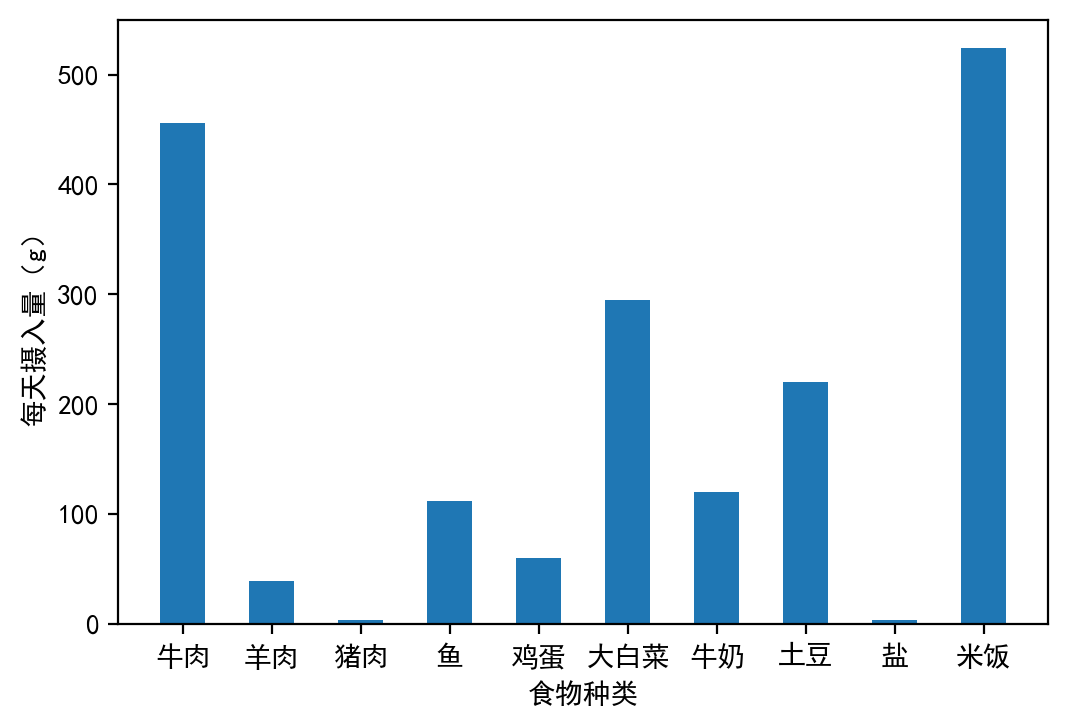
\includegraphics[width=0.6\linewidth]{figures/fig2.png}
	\caption{摄入量柱状图}
	\label{boxplot-fig}
\end{figure}

\begin{figure}[h!]
	\centering
	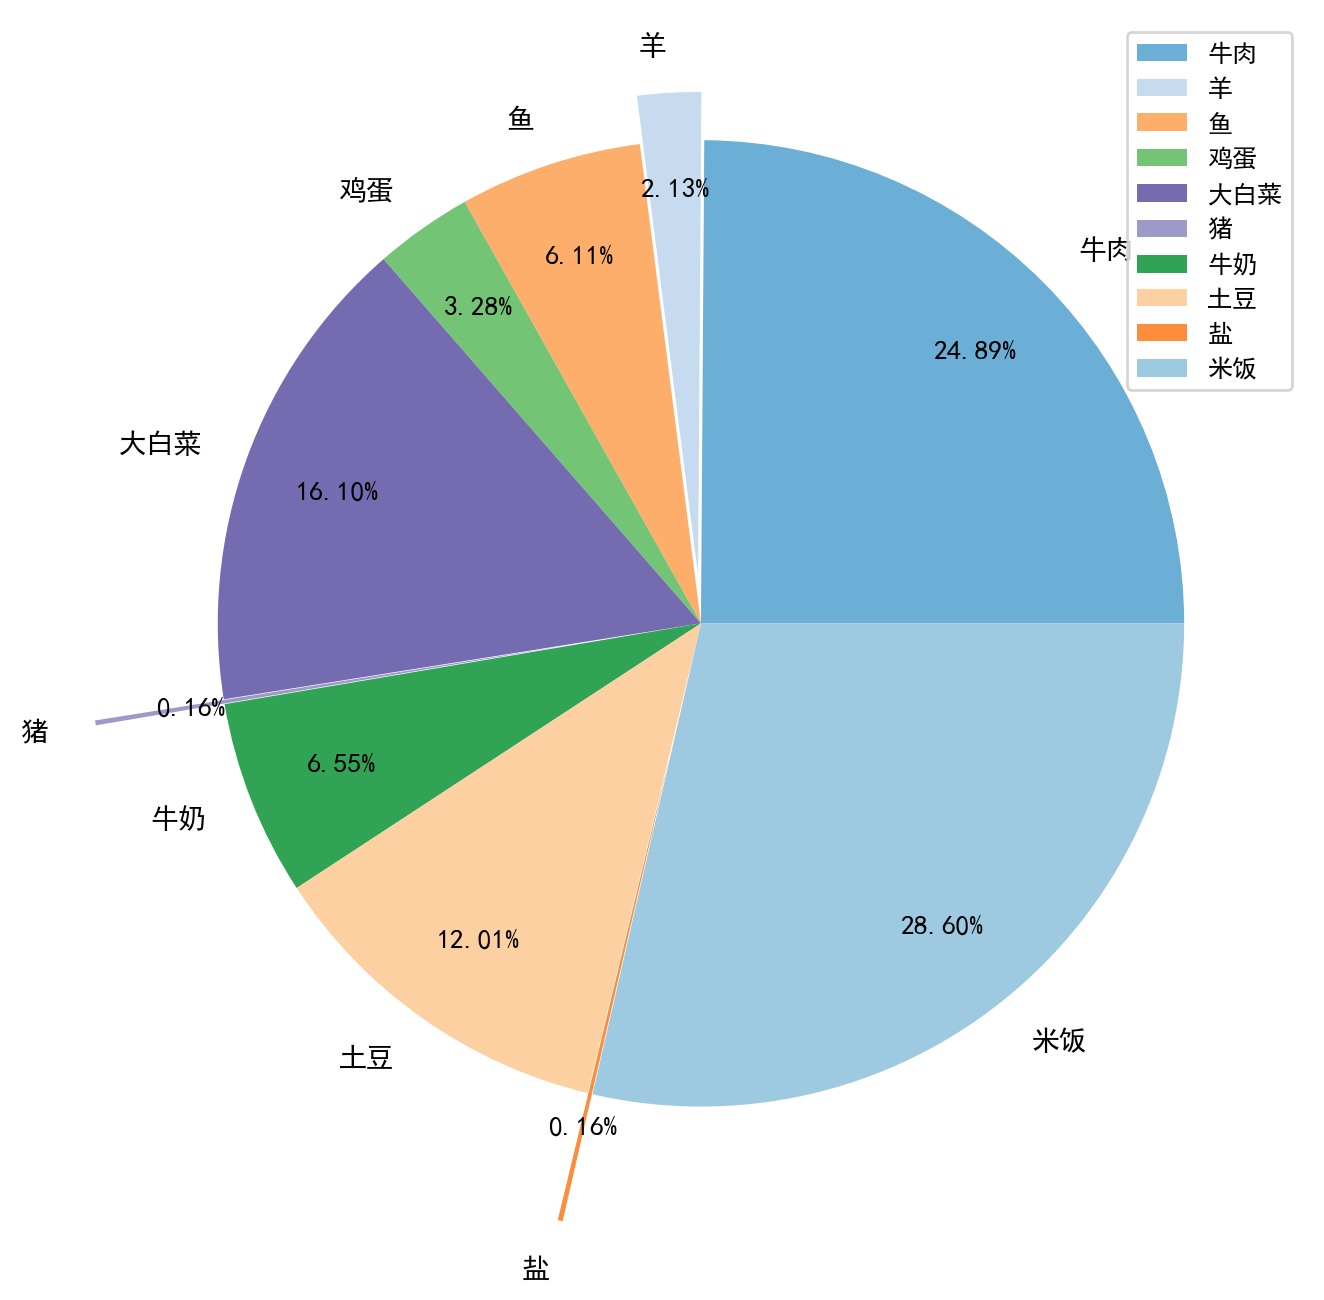
\includegraphics[width=0.6\linewidth]{figures/fig3.png}
	\caption{摄入量占比图}
	\label{pieplot-fig}
\end{figure}
根据图\ref{boxplot-fig}和\ref{pieplot-fig},我们可以发现,人一天中摄入量最大的是米饭和牛肉,大米能给人提供足够的基本营养物质。而牛肉的摄入量也较高,因为牛肉能在同样的热量下提供更多的蛋白,单位营养价值较高。人体大白菜需求占比也很高,因为大白菜含有较多维生素,维生素是人类生理活动非常关键的微量元素。最后,由上面的图可见,人类在日常饮食中要追求荤素平衡,在营养、能量足够的同时补充足够的维生素,让身体更健康。

\section{模型灵敏度分析}
灵敏度分析是研究与分析一个数学模型输出变化对模型输入参数的敏感程度的方法。在最优化方法中经常利用灵敏度分析来研究原始数据不准确或发生变化时最优解的稳定性。通过灵敏度分析还可以决定哪些参数对系统或模型有较大的影响。

本题目中的变量有人的\textbf{身高、体重、性别和年龄},这几个变量决定一个人的BMR值,从而影响多目标规划的决策结果。这里,可以微调上面的几个变量,观察决策结果(每种食物的建议摄入量)的变化幅度来分析本模型的灵敏度。

我使用了以下几个参数进行试验,得到结果如表\ref{every-person-intake-table}所示。

A人:性别男,体重70kg,身高180cm,年龄20岁

B人:性别男,体重72kg,身高178cm,年龄22岁

C人:性别男,体重66kg,身高174cm,年龄24岁
\begin{table}[h!]
\centering
\renewcommand\arraystretch{0.65}
\begin{tabular}{ccccccccccc}
\toprule
人 & 牛肉 & 鸡肉 & 猪肉 & 鱼 & 水果 & 大豆类 & 其他 & 乳品 & 酒 & 米饭 \\
\midrule
A & 461g & 39g & 3g & 114g & 61g & 295g & 122g & 222g & 3g & 530g \\
B & 461g & 39g & 3g & 115g & 61g & 295g & 128g & 222g & 3g & 531g \\
C & 437g & 35g & 3g & 111g & 60g & 296g & 119g & 212g & 3g & 504g \\
\bottomrule
\end{tabular}
\caption{A, B, C每个人推荐食物摄入量表}
\label{every-person-intake-table}
\end{table}

下面画出三个人推荐摄入量的散点图,便于观察几种人体参数下食物推荐摄入量的差距:
\begin{figure}[h]
	\centering
	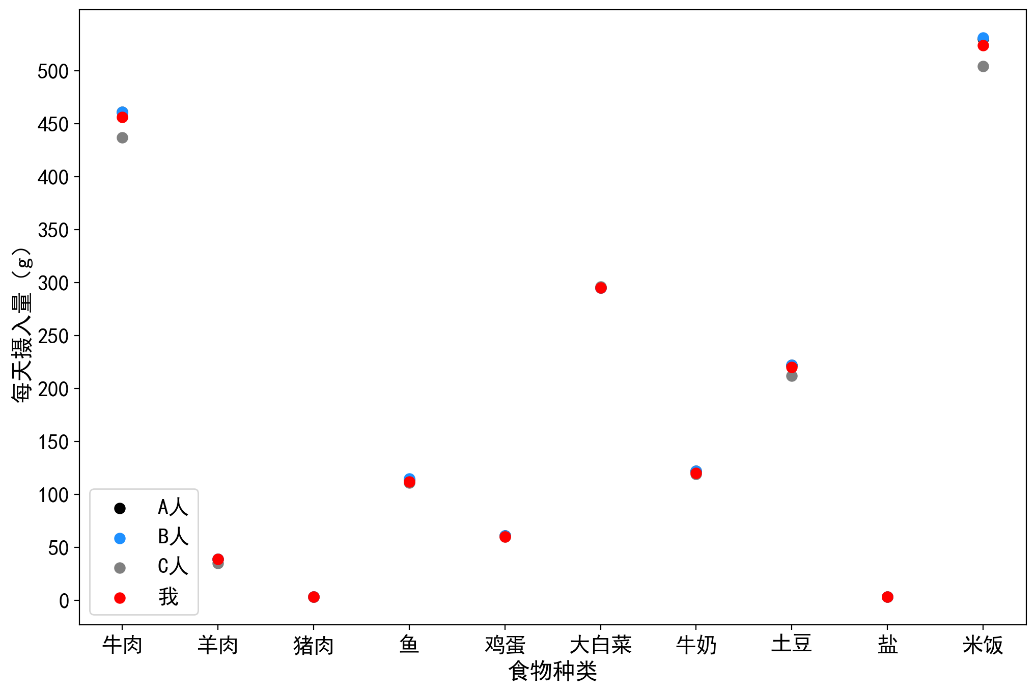
\includegraphics[width=0.7\textwidth]{figures/fig4.png}
	\caption{推荐食物摄入量散点图}
	\label{scatter-fig}
\end{figure}

根据如上的结果,在微调人体各变量的情况下,每种食物的建议摄取量没有出现过大的变化,只是一部分的食物摄入量出现极小的变化,其他的摄入量有时甚至没有变化。因此,这个模型的稳定性较好。

\section{模型的不足}

\subsection{建模方法中的问题}

这次的建模中,我选择了优先级法来对模型中的多目标规划问题进行求解,这在一定程度上简化了问题,使我能够使用单目标规划的方法求解。但是这样也忽略了多个决策目标之间的关系,使得出的结果有较大的不准确和主观性。

此处各个决策目标之间的关系是我自己人为设定的,是较为主观的,与实际情况可能不相符。这种设定各目标之间优先级的方法不够准确,可能由于我个人判断的失误导致模型求解结果的误差。

\subsection{建模所用数据量和准确性问题}

为了建模计算过程和计算量的简化,我只考虑了10种常见的食物,使用的数据量较少。而人日常的食物摄入品种应该是远远丰富于此的,在后续的优化中需要添加更多的食品种类。

同时,建模中使用的数据也不是完全准确的,有的食物中营养素含量过少,在填入表格的时候直接填0处理,建模求解的结果也会因此跟真实值有微小的差别,在后续可以考虑将填0的数据改为精确值,提高模型精度。

% =============================================
% Part 5: 参考文献
% =============================================
%在reference.bib文件中填写参考文献,此处自动生成

%\newpage
\bibliographystyle{ieeetr}
\clearpage
\phantomsection
\addcontentsline{toc}{section}{参考文献} %向目录中添加条目,以章的名义
\bibliography{reference.bib}
\end{document}